\section{bpred\_\-taken\_\-t Class Reference}
\label{classbpred__taken__t}\index{bpred\_\-taken\_\-t@{bpred\_\-taken\_\-t}}
Inheritance diagram for bpred\_\-taken\_\-t:\nopagebreak
\begin{figure}[H]
\begin{center}
\leavevmode
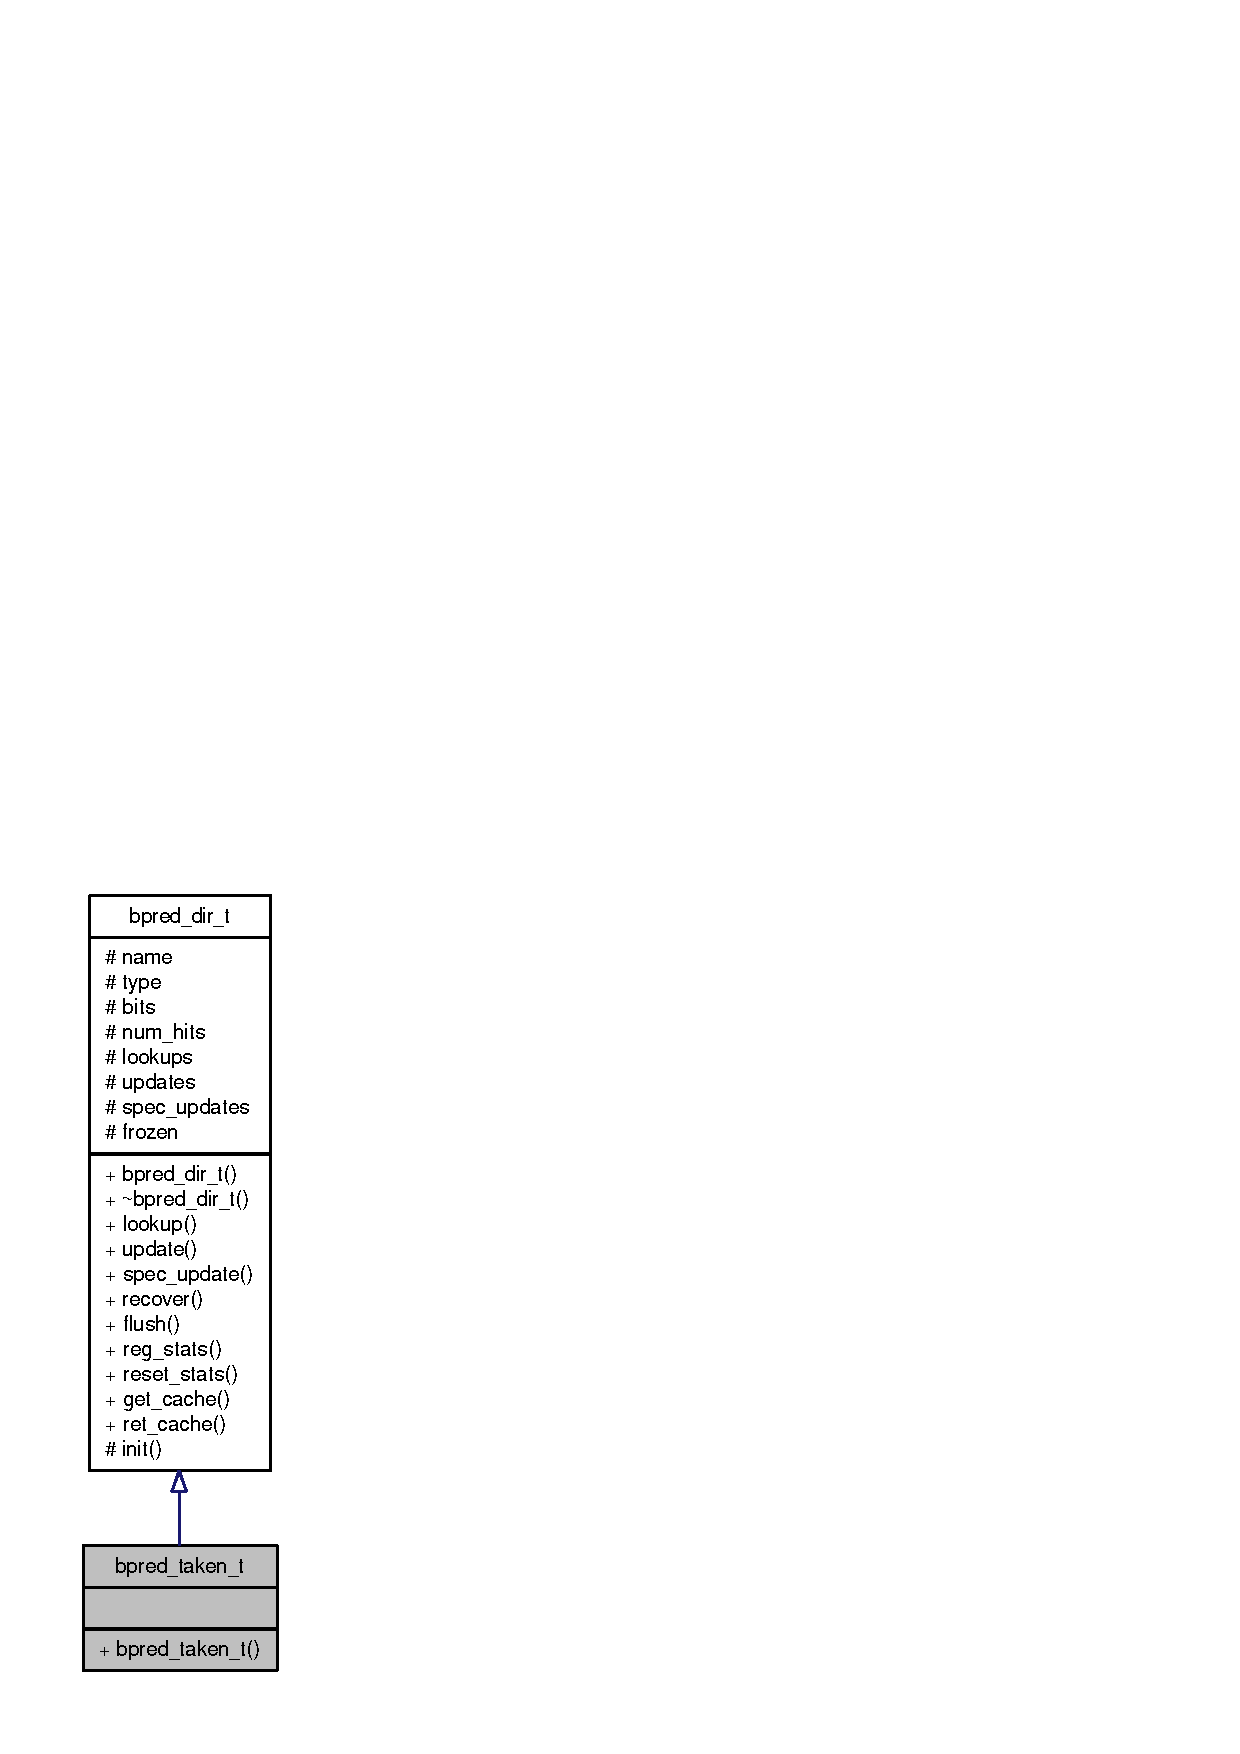
\includegraphics[height=400pt]{classbpred__taken__t__inherit__graph}
\end{center}
\end{figure}
Collaboration diagram for bpred\_\-taken\_\-t:\nopagebreak
\begin{figure}[H]
\begin{center}
\leavevmode
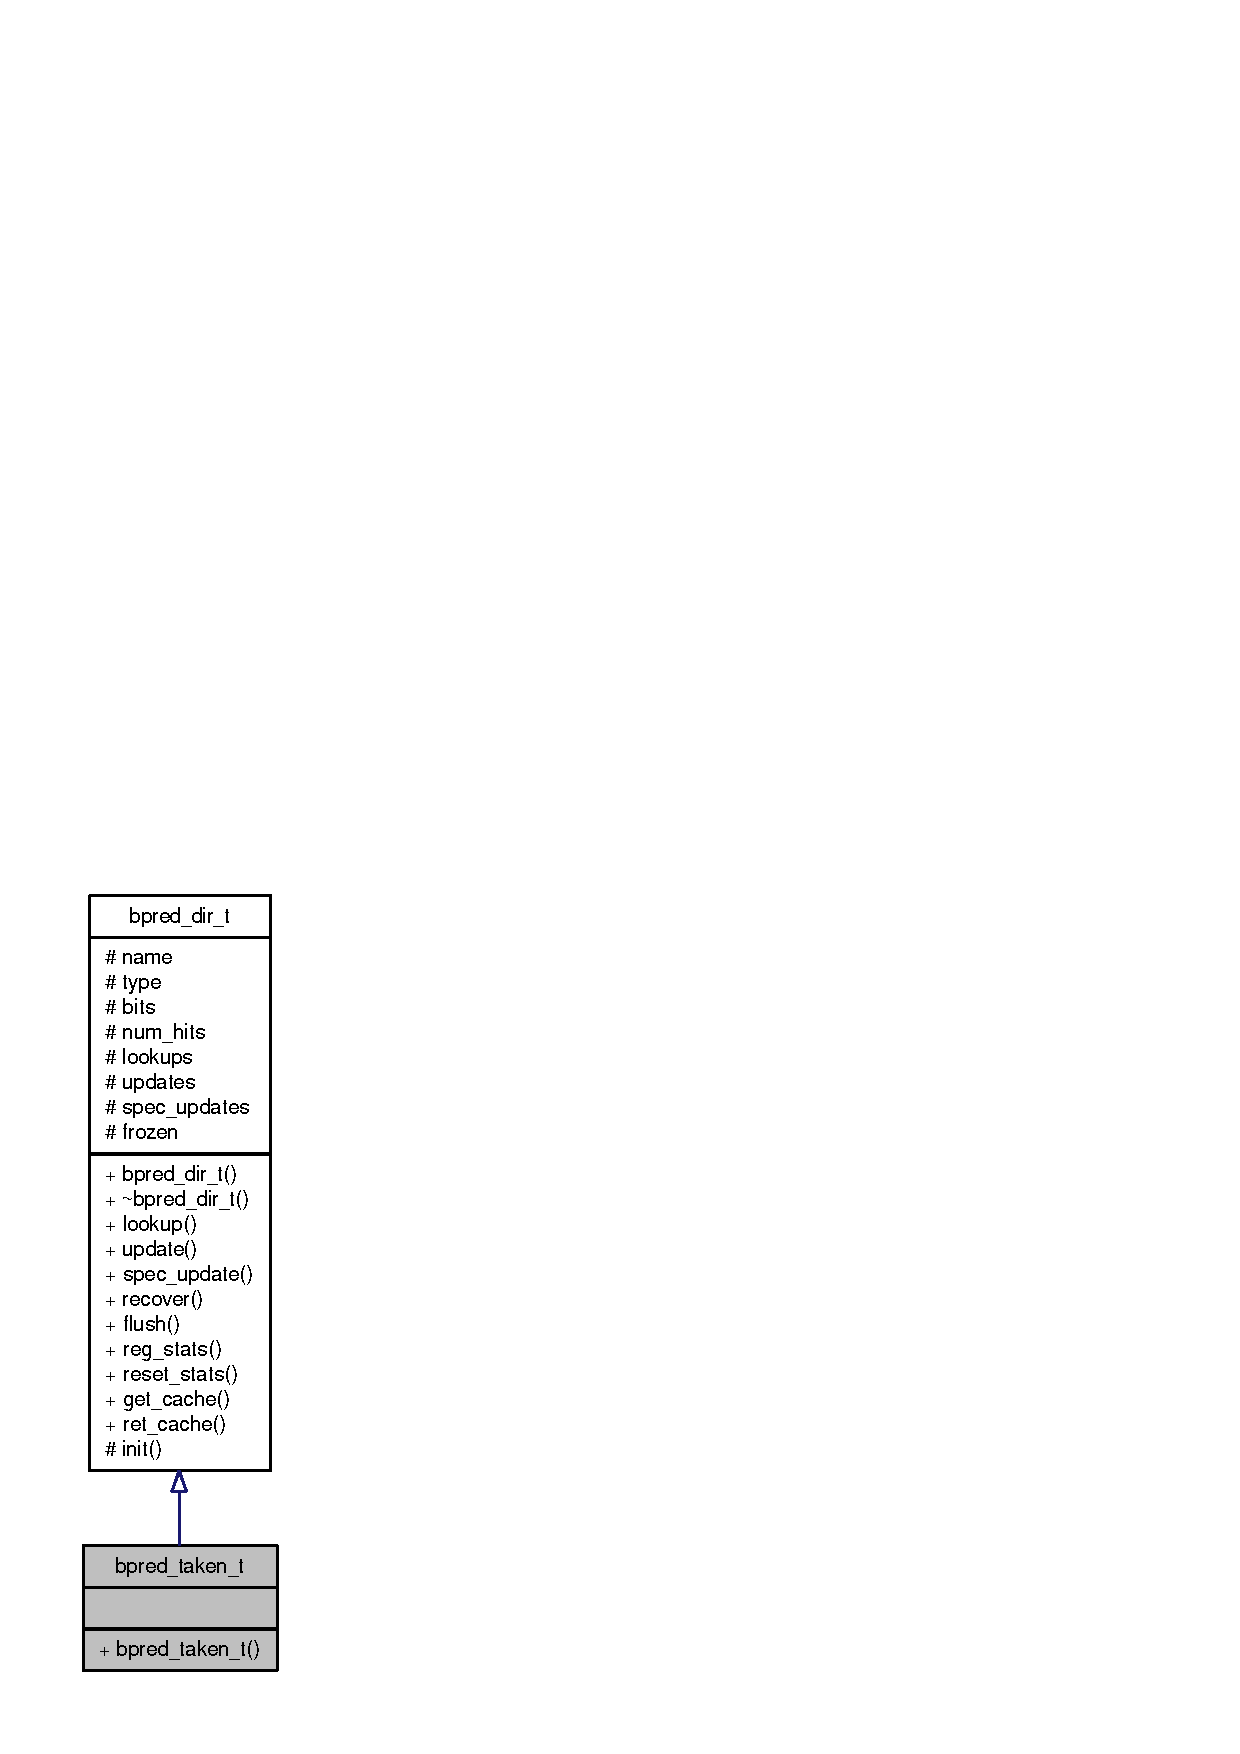
\includegraphics[height=400pt]{classbpred__taken__t__coll__graph}
\end{center}
\end{figure}
\subsection*{Public Member Functions}
\begin{CompactItemize}
\item 
{\bf bpred\_\-taken\_\-t} ()
\end{CompactItemize}


\subsection{Detailed Description}


Definition at line 15 of file bpred-taken.cpp.

\subsection{Constructor \& Destructor Documentation}
\index{bpred\_\-taken\_\-t@{bpred\_\-taken\_\-t}!bpred\_\-taken\_\-t@{bpred\_\-taken\_\-t}}
\index{bpred\_\-taken\_\-t@{bpred\_\-taken\_\-t}!bpred_taken_t@{bpred\_\-taken\_\-t}}
\subsubsection[{bpred\_\-taken\_\-t}]{\setlength{\rightskip}{0pt plus 5cm}bpred\_\-taken\_\-t::bpred\_\-taken\_\-t ()\hspace{0.3cm}{\tt  [inline]}}\label{classbpred__taken__t_73d4a924c1feb9fd4002b270aad7ab24}




Definition at line 20 of file bpred-taken.cpp.

References bpred\_\-dir\_\-t::bits, COMPONENT\_\-NAME, fatal(), bpred\_\-dir\_\-t::init(), bpred\_\-dir\_\-t::name, and bpred\_\-dir\_\-t::type.

The documentation for this class was generated from the following file:\begin{CompactItemize}
\item 
{\bf bpred-taken.cpp}\end{CompactItemize}
